\documentclass{article}
\usepackage{amsmath}
\usepackage{slashed} % for slash ET
\usepackage{graphicx}
\title{E214 questions}
\begin{document}
\maketitle
\section{Section 7.2.2}
Question A: Decay of the $Z^0$ boson\\
\textit{Which value does the momentum of an electron have in the decay of a $Z^0$ boson $Z^0 \, \rightarrow \, e^+ e^-$, if the $Z^0$ is at rest?}\\
\par From four-momentum conservation:
\begin{align*}
p_{Z^0} &= \begin{bmatrix}
           m_{Z^0} \\
          \vec{0} \\
         \end{bmatrix} 
         =
         \begin{bmatrix}
         E_e\\
         \vec{p}
         \end{bmatrix}
         +
         \begin{bmatrix}
         E_e\\
         -\vec{p}
         \end{bmatrix}
         = p_{e^+} + p_{e^-} \nonumber
\intertext{From this, we get}
m_{Z^0} &= 2 \sqrt{p^2 + m_e^2} = 91.2 \, \text{GeV}, \hspace{6pt} m_{e} = 511 \, \text{GeV}\\[8pt]
\Rightarrow p &= \sqrt{\frac{m_{Z^0}^2}{4} - m_e^2} = 45.6 \, \text{GeV}
\end{align*}\\
Question B: Scattering reaction $e^+ e^- \, \rightarrow \, \tau^+ \tau^-$\\
\textit{How large is the momentum of tau leptons in the reaction $e^+ e^- \, \rightarrow \, \tau^+ \tau^-$, if the reaction takes place in the center-of-mass system (center-of-mass energy = 5~GeV)?}\\
\par In CMS frame ($\vec{p}_{e^-} = - \vec{p}_{e^+}$), the energy squared:
\begin{align*}
s = (p_{\tau^+} + p_{\tau^-})^2 &= \begin{bmatrix}
2E_{\tau}  \\
\vec{0}
\end{bmatrix}^2 = 4 E_{\tau}^2 = E_{CMS}^2=25 \, \text{GeV}^2 
\end{align*}
We can calculate ($m_\tau \approx 1.78$~GeV) the three-momentum of the tau leptons:
\begin{align*}
p_{\tau}^2 = E_{\tau}^2 - m_{tau}^2 &= \Big( \frac{25}{4} - 1.78^2 \Big) \, \text{GeV$^2$}\\[8pt]
p &= 1.755 \, \text{GeV}
\end{align*}
\section{Section 7.4.1}
\textit{How could the variable \texttt{ptw} be constructed from other tree variables?}\\
\par We are looking at $W \, \rightarrow e \nu$ processes. We can use the missing transverse momentum (\texttt{ptmis\_x, ptmis\_y}), which we assign to the neutrino. As we know the electron transverse momentum: \texttt{el\_px, el\_py, el\_pt}, the W-boson transverse momentum is determined by momentum conservation, if the \\[14pt]
\textit{The correct form of the Gauss error propagation law in the presence of correlations.}\\
%Barlow pp. 58-60 (4.11-12)
\par The standard deviation squared of a function $f(x,y)$ is given by
\begin{equation}
\sigma_f^2 = \Big(\frac{df}{dx}\Big)^2 \sigma_x^2 + \Big( \frac{df}{dy} \Big)^2 \sigma_y^2 + 2 \frac{df}{dx}\frac{df}{dy}\text{cov}(x,y)
\end{equation}
\section{Section 7.5.1}
\textit{What is the minimum invariant 4-lepton-mass, when the four leptons originate from a $Z^0$ pair? Why do you find 4-lepton-events with invariant mass beneath this threshold?}\\
\par At threshold, the $Z^0$ boson decays at rest, in this case: $m_{Z^0} = 2 m_l$. The minimum 4-lepton invariant mass is acquired when both $Z^0$'s are stationary (CMS frame),and equal to $2m_{Z^0}$. When one or two of the $Z^0$ bosons is off-shell, the 4-lepton-mass can be lower than $2 m_{Z^0}$. \\[14pt]
\textit{Consider a Higgs boson which decays into two $Z^0$ bosons. How does the distribution of the 4-lepton-invariant-mass look like?}\\
\begin{figure}
\centering
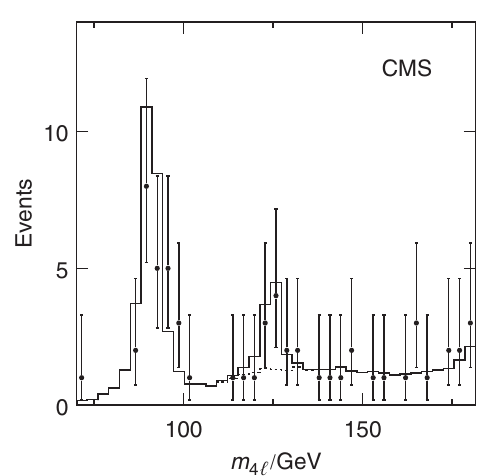
\includegraphics[scale=0.5]{Images/Z0peak.png}
\caption{The invariant 4-lepton-mass distribution. \textit{Thompson: Modern Particle Physics Fig. 17.19}}
\end{figure}
%See manual p. 41, also Thomson 17.19
\par There is a $Z^0$ peak (at $\approx 90$~GeV) and a Higgs-boson peak (at $\approx 125$~GeV). These come from the $Z^0 \, \rightarrow \, 4\ell$ and the $H^0 \, \rightarrow \, Z Z \, \rightarrow 4 \ell$ processes, respectively.  One example for the background at the Higgs-peak is the $t \rightarrow bW^+$ decay.\\[14pt]
\textit{Assume you have an ideal detector. What is the typical $\slashed{E}_T$ if a $Z^0$ pair has been produced and both $Z^0$ decay into electron or muon pairs? What $\slashed{E}_T$ will you expect when you have a real detector?}\\
\par In an ideal detector, there would be no missing energy in this process. In real detectors, there are energy losses not detected due to inactive detector elements, imperfect calibration.\\[14pt]
\textit{The Branching ratio of $t \, \rightarrow \, Wb$ is almost 100\%. If you have a top anti-top pair in an event, both particles decay instantly via $t \, \rightarrow \, bW$. If both W bosons each decay leptonically ($W \, \rightarrow \, \ell \nu$), one finds two leptons in the event. What could explain the occurence of four leptons in a $t \bar{t}$ event?}\\
\par The two top quarks can decay into b quarks and W bosons, both of which can further decay semi-leptonically. The process: 
\begin{equation}
t \bar{t} \, \rightarrow bW^+ \, \bar{b}W^- \, \rightarrow (l^- \ldots ) \, (\nu l^+) \, (l^+ \ldots) \, (l^- \bar{\nu})\nonumber
\end{equation}\\
\textit{Gedanken-experiment: given a histogram with 2000 bins of 20000 random integers between 1 and 2000, we expect an average of 100 entries per bin. What is the statistical error for the number of entries in one bin? What is the probability of finding a bin with 130 entries? How many of such 130 entries bins (in average) do you expect to appear in 200 bins? In other words, what is the probability to find a deviation of 3 standard deviations in one of the bins of the distribution?}\\
\par The error for bin entries is (counting statistics) $\sqrt{100} = 10$. Finding a bin with 130 entries (or more): $\sigma = 10 \Rightarrow 3\sigma$ is what we are looking for. The probability of higher than 130 or lower than 70 is $ 1- 3 \sigma = 1-0.9973$, so the requested probability for 1 bin is $(1-3\sigma)/2$. The probability that at least one of the bins has more than 130 counts:
\begin{equation}
P = 1 - \Big( 1 - \frac{1- 0.9973}{2} \Big)^{200} = 1-0.7532 = 0.2368.
\end{equation} 
\end{document}